%----------------------------------------
%               Essential    
%----------------------------------------
\documentclass[12pt]{article}
%-----------------------------------------------
%        Hugos Template - V. 2021.04.09
%-----------------------------------------------
%                   Settings
%-----------------------------------------------
%   Ändra språk, och snabb compile
\usepackage[english, provide=*]{babel}       % Språk. [swedish] eller [english].
\usepackage[]{graphicx}           % Bilder. [demo] för snabb compile!

%   Extra
%\usepackage{mhchem}    % Kemiekvationer.
%\usepackage{changepage}           % Lokal ändring i margin, \begin{adjustwidth}{-1cm}{-1cm}


%-----------------------------------------------
%                   Packages
%-----------------------------------------------
\usepackage[utf8]{inputenc}          % Kodning av text.
\usepackage[]{biblatex}              % (Vancouver), \cite \textcite
%..[style=authoryear-ibid]           % (Harvard), \parencite \textcite
%..[style=apa]                       % (APA) \textcite \parencite
%\DeclareLanguageMapping{swedish}{swedish-apa}


\pagenumbering{gobble}       % Stoppar sidnumrering på titelsida.
\usepackage{mathtools}       % Ekvationer.
\usepackage{bm}              % Bold matte
\usepackage[]{geometry}      % Sidlayout.
\usepackage{float}           % För [H].
\usepackage[T1]{fontenc}     % Bra för åäö.
\usepackage{csquotes}        % Fancy Quotes
\usepackage[expansion=false]{microtype}       % Fixar bättre textlayout.

\usepackage[margin=15pt,font={small},labelfont={bf}%
,justification=centering]{caption}      % Snygg figurtext.
\usepackage{booktabs}                   % Snygga Tabeller.
\usepackage{longtable}                  % Långa tabeller, flera sidor.
\setlength{\abovecaptionskip}{3pt}      % Flyttar tabelltext närmare.
\renewcommand{\arraystretch}{1.2}       % Gör tabeller  större.
\setlength{\parindent}{0cm}             % Tar bort "indent" på ny rad.
\usepackage[none]{hyphenat}             % Slutar dela upp ord.

\bibliography{Essential/References.bib} % Mapp för Källor.
\graphicspath{{Images/}}                % Mapp för bilder.
\usepackage{pgffor}                     % Loop för bilagor.
\usepackage{pdfpages}                   % PDFs.
\usepackage{tikz}                       % TikZ diagrams.
\usetikzlibrary{positioning, arrows.meta, shapes}  % TikZ libraries.
\addto{\captionsswedish}{\renewcommand*%%
{\contentsname}{Innehållsförteckning}}  % Ändrar namn -> Innehållsförteckning

\usepackage[colorlinks]{hyperref}                  % Hyperlänkar + färg.
\usepackage[nameinlink,noabbrev,swedish]{cleveref} % \cref{} & \Cref{}.
\usepackage{color}                                 % Färg.
\definecolor{royalblue}{rgb}{0.0, 0.14, 0.4}       % Egen färg.
\hypersetup{                                       % Färg på hyperlänkar.
     colorlinks  = true,
     linkcolor   = black,              % internal links.
     citecolor   = royalblue,          % bibliography.
     filecolor   = royalblue,          % file links.
     urlcolor    = royalblue           % external links.
}

% \usepackage{matlab-prettifier}          % Matlab text!
\usepackage[per-mode=symbol]{siunitx}   % si. Skriva enheter/nummer.
\sisetup{output-decimal-marker={,},%    % si. ("{,}" till "{.}" för engelska).
range-phrase=--,range-units=single,exponent-product=\cdot}

%-----------------------------------------------
%                 New commands                
%-----------------------------------------------
% Använd för radbyte. \n
\newcommand{\n}{\vskip 1em}

% Bold matte och text (Automatisk) ex. \B{TEXT och } $\B{\alpha}$
\newcommand*{\B}[1]{\ifmmode\bm{#1}\else\textbf{#1}\fi}

% Partial Derivative. \pde{a}{b}
\newcommand{\pde}[2]{\frac{\partial #1}{\partial #2}}

% Använd för matlab fil.
\newcommand{\matlabfile}[1]
{\UseRawInputEncoding\hyphenpenalty=50\exhyphenpenalty=50\lstinputlisting[style = Matlab-editor,basicstyle = \mlttfamily]{#1}}

% Använd för matlab text.
% \lstnewenvironment{matlab}
% {\UseRawInputEncoding\hyphenpenalty=50\exhyphenpenalty=50\lstset{style = Matlab-editor,basicstyle = \mlttfamily}}{}

\usepackage[page,toc,titletoc,title]{appendix}

% Kollar om det finns .tex fil Från Bilaga_1 till Bilaga_15.
% Genererar sida om det finns. Öka från 15 vid behov.
\edef\bilagamax{15}
\newcommand{\bilagaloop}{\foreach \i in {1, 2, 3, ...,\bilagamax} {
    \edef\FileName{Sections/Bilagor/Bilaga_\i}%
    \IfFileExists{\FileName.tex}{%
        \newpage%
        \section{}%
        \input{\FileName.tex}%
    }{}
}\IfFileExists{Sections/Bilagor/Bilaga_\bilagamax.tex} {\errmessage{MAX ANTAL BILAGOR, ÖKA "bilagamax" i Packages.tex}}
}

%%%%%%%%%%%%%%%%%%%%%%%%%%%%%%%%%%%%%%%%%%%%%%%%%%%%
%%  Creative Commons CC BY 4.0, Hugo Laestander %%%%
%%%%%%%%%%%%%%%%%%%%%%%%%%%%%%%%%%%%%%%%%%%%%%%%%%%%
%-----------------------------------------------
%            Titelsida, ändra dessa!
%-----------------------------------------------
% Style
%  Max 7 pers totalt  -> Titlestyle_Big
%  Max 10 pers totalt -> Titlestyle_Small
%  Ingen bild         -> Titlestyle_Text
\def\thetitlestyle{Titlestyle_Big}
%-----------------------------------------------

% Titel
\def\thetitle{Hyperledger Fabric}
\def\thesubtitle{Ett distribuerat operativsystem för behörighetsstyrda blockkedjor,\\D7024E semenarium}


% Kurs
\def\thecoursename{Grupp 12}


% Författare
\def\theauthor{
Adrian Fingal & adrfin-1@student.ltu.se \\
Oscar Johansson & osajoh-9@student.ltu.se\\
Hugo Hedlund & hughed-0@student.ltu.se
}

% Handledare
\def\thesupervisor{\href{https://dl.acm.org/doi/pdf/10.1145/3190508.3190538}{Hyperledger Fabric Whitepaper}}

% Institution
\def\theinstitution{Institutionen för system- och rymdteknik}

% Logga
\def\thelogo{LTU_swe.jpg}

\begin{document}
\input{Essential/Style/\thetitlestyle}
\restoregeometry
\tolerance=2000
\pagenumbering{roman}
\setcounter{page}{1}

%-----------------------------------------
%                Sections
%-----------------------------------------
% Skriv direkt i filerna i /Sections/...
% Ändra nedanstående kod vid behov.
%-----------------------------------------

\newpage
\tableofcontents
\hypersetup{linkcolor=royalblue}

% \newpage
% \section*{Beteckningar}
%
\vspace{-5mm}
\begin{longtable*}[l]{@{} l l l @{}}
\toprule\endfirsthead
\B{Symbol} & \B{Benämning} & \B{Enhet} \\
\midrule
    $E$ & Energi & \si{\J} \\
    $m$ & Massa & \si{\kg} \\
    $c$ & Ljusets hastighet & \si{\m\per\s} \\
\bottomrule \\
\end{longtable*}

\newpage
\pagenumbering{arabic}


\section{Frameworks}
In this section, we will discuss the various frameworks and technologies that are being utilized in the project. This includes both the backend and frontend technologies, as well as any other tools that are essential for the development process.

\begin{list}{}
    \item \textbf{Programming language:} Go is used as the primary programming language for the backend services, leveraging its concurrency features and performance.
    \item \textbf{Logging:} Logrus is used for structured logging in the application, providing a simple API for logging that allows to pass the container ip address for each log entry to easily identify which node the log entry originated from.
    \item \textbf{Containerization:} Docker in swarm mode is used for container orchestration, enabling the management of multiple containers.
    \item \textbf{Automation:} Bash scripts are employed to automate common tasks such as building and deploying the application, making it easier to manage the deployment and development process.
\end{list}
\newpage

\section{Sprints}

\subsection{Organizing Sprints}

To structure and organize the work efficiently, GitHub Projects is used to create a storyboard for both sprints. The storyboard is available under the 
Projects tab in the repository, providing an overview of the workflow throughout the course.

\subsection{Sprint 0}
\subsubsection{Done in sprint 0}
During sprint 0 we setup the project repository from the Github template given in the course. We also configured a containerization strategy using Docker in swarm mode. We established bash scripts to automate common tasks, such as building and deploying the application. This lets us with a simple script deploy up to n instances, where n is a argument for the deploy script, with ease. Utilizing these scripts, we can easily scale up and down the number of instances in our swarm and Kademlia network in the upcoming sprints.

After setting up the containerization tools, we started on the implementation of finding nodes in the same docker network and establishing communication between them. Our approach involved DNS lookups via the docker DNS service, to get the docker ip addresses of the other containers in the same docker swarm stack. The drawback of this approach is that the containers that start up early won't be able to find the containers that start up later, since they don't exist yet. We didn't solve this problem yet, as we will implement Kademlia protocol for peer discovery to address these issues later in the sprint.
    
\subsubsection{Plan for sprint 0}
In sprint 0, we plan to focus on the following tasks:
\begin{itemize}
    \item \textbf{M1} Implement the Kademlia protocol for pinging
    \item \textbf{M1} Implement the Kademlia protocol for network joining
    \item \textbf{M1} Implement the Kademlia protocol for finding nodes
    \item \textbf{M1} Create unit tests for the implemented Kademlia functionalities, via mocking
\end{itemize}

\subsection{Sprint 1}

\subsubsection{Planned work}

As illustrated in Figure \ref{fig:todos_for_sprints_at_sprint_0}, the plan is to complete all underlying functionality (M2-M7) during sprint 1.
Subsequently, focus will shift to the qualification goals (U1–U5), during sprint 2. This structure was chosen because establishing and verifying the core functionality 
first ensures a stable foundation, which in turn facilitates the successful implementation of the qualification objectives.


\newpage
\section{System Architecture}

\subsection{Implementation Overview}

While implementing the Kademlia DHT, our focus was to create a modular and extensible system, that can easily be maintained and expanded upon in the future.
To achieve this, we sought to seperate out as many components as possible, keeping each file and package focused on a single responsibility, while also utilizing 
handlers to abstract away the underlying implementation details of each component. This approach allows us to easily swap out components, such as the network layer, 
without affecting the rest of the system.

\subsection{Implementation Details}
One important aspect of our implementation is how we handle docker swarm mode to spin up multiple instances of our Kademlia node and form a network. Each node needs to know the IP address and the ID of a node to join the network via that node. To facilitate this, we chose to use a bootstrap node, which is a already known node in the network that all subsequent nodes can connect to. This bootstrap node is started first, and has a hard coded ID in the docker compose file, but can easily be exchanged for any other ID by changing the docker compose fil to use a environment variable instead. All other nodes are then started and knows the docker service name of the bootstrap node and gets its ID via a CLI flag when started. This way, all nodes can connect to the bootstrap node and join the network.



\subsection{System Architecture Diagram}
A high level system architecture diagram is shown in Figure \ref{fig:architecture}. The diagram illustrates the main components of the Kademlia system and some of their interactions. Note, this is a simplified view of the system and does not include all components and interactions. The main components are described below:
\begin{itemize}
    \item \textbf{Network Layer:} This layer handles all network communications, including sending and receiving messages between nodes. It abstracts away the underlying network implementation, allowing for easy replacement or modification. As of now, there exists a mock network implementation for testing purposes as well as a UDP based implementation for actual network communication.
    \item \textbf{Kademlia Node:} This component represents a single node in the Kademlia network. It manages its routing table, handles incoming requests, and initiates outgoing requests to other nodes.
    \item \textbf{Routing Table:} The routing table is responsible for maintaining a list of known nodes in the network. It organizes nodes into buckets based on their distance from the current node, facilitating efficient lookups and routing. This implementation does not implement the correct binary tree structure as described in the Kademlia paper, but rather uses a simpler list based approach for storing nodes in each bucket (given by the lab instructions).
    \item \textbf{Message Handlers:} These components are responsible for processing incoming messages and executing the appropriate actions based on the message type (e.g., PING, STORE, FIND VALUE). There also exsists temporary message handlers which are used for waiting for responses to outgoing requests, such as waiting for a PONG response after sending a PING request. These temporary handlers are removed once the response is received or a timeout occurs. But they are removed from the diagram for simplicity.
    \item \textbf{Command Line Interface (CLI):} The CLI provides an interactive interface for users to interact with the Kademlia node, allowing them to execute commands such as joining the network, storing values, and retrieving values.
    
\end{itemize}

\begin{figure}[htbp]
    \centering
    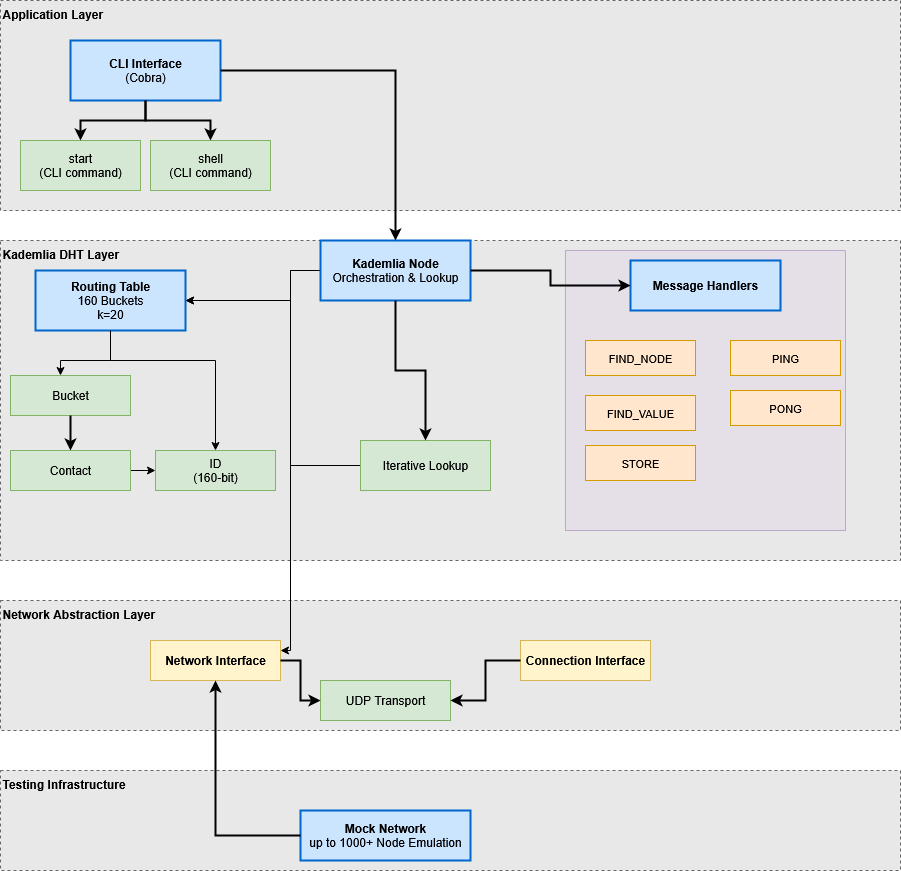
\includegraphics[width=0.8\textwidth]{Images/component_diagram.drawio.png}
    \caption{Component diagram of the Kademlia DHT system showing the layered architecture and component relationships.}
    \label{fig:architecture}
\end{figure}


% \section{Sprint 2}
% \newpage



\newpage
% \printbibliography

%-----------------------------------------
%                 Bilagor
%-----------------------------------------
% Skapa nya filer i "Sections/Bilagor/"
% som heter Bilaga_1.tex, Bilaga_2.tex,..
% Så läggs de in automatiskt! :)
%-----------------------------------------

\IfFileExists{Sections/Bilagor/Bilaga_1.tex}{
% \begin{appendices}
%     \bilagaloop
% \end{appendices}
}{}
\end{document}